% !TEX options=-shell-escape
\documentclass[12pt]{article}
\setlength{\parskip}{1em} % 设置段落之间的间距
\setlength{\parindent}{8pt} % 全局取消段首缩进


\usepackage{fancyhdr}
\usepackage{lastpage}
\usepackage{amsthm}
\usepackage{hyperref}
\usepackage{amsmath}
\usepackage{amsfonts}
\usepackage{siunitx}
\usepackage{footnote}
\usepackage{tablefootnote}
\usepackage{makecell}
\usepackage[letterpaper, left=2cm,right=2cm,top=3cm,bottom=2cm]{geometry}
\usepackage{longtable}
\usepackage{multirow}
\usepackage{array}
\usepackage{verbatim}
% \usepackage{unicode-math}
\usepackage{minted}
\usepackage{booktabs}
\usepackage{algorithm}
\usepackage{algpseudocode}
\usepackage{subcaption}
\usepackage{graphicx}
\usepackage{tocbibind}
\usepackage[toc,page]{appendix}
\usepackage[]{mhchem}
\usepackage{setspace}
\usepackage{placeins}
\usepackage[]{pdfpages}
\usepackage{indentfirst}
\usepackage{listings}

% \newcommand{\setParDis}{\setlength {\parskip}{0.3cm}}
% 
% \setmathfont{XITS Math}
% \setcounter{tocdepth}{2}
\setlength{\parskip}{0.5em}
% \numberwithin{equation}{subsection}
% \newcommand{\upcitep}[1]{\textsuperscript{\textsuperscript{\citep{#1}}}}

\DeclareMathOperator*{\argmax}{arg\,max}
\DeclareMathOperator*{\argmin}{arg\,min}
\DeclareMathOperator*{\var}{Var}

\newtheorem{assumption}{Assumption}
\newtheorem{definition}{Definition}
\newtheorem{question}{Question}

\pagestyle{fancy}
\fancyhf{}
\rhead{Page \thepage\ of \pageref{LastPage}}
\lhead{Team \# 15607}



\usepackage{geometry}
\geometry{left=1in,right=0.75in,top=1in,bottom=1in}

%%%%%%%%%%%%%%%%%%%%%%%%%%%%%%%%%%%%%%%%
% Replace ABC in the next line with your chosen problem
% and replace 1111111 with your Team Control Number
\newcommand{\Problem}{A}
\newcommand{\Team}{15607}
%%%%%%%%%%%%%%%%%%%%%%%%%%%%%%%%%%%%%%%%

\usepackage{newtxtext}
\usepackage{amsmath,amssymb,amsthm}
\usepackage{newtxmath} % must come after amsXXX

\usepackage[pdftex]{graphicx}
\begin{document}
\graphicspath{{.}}  % Place your graphic files in the same directory as your main document
\DeclareGraphicsExtensions{.pdf, .jpg, .tif, .png}
\thispagestyle{empty}
\vspace*{-16ex}
\centerline{\begin{tabular}{*3{c}}
	\parbox[t]{0.3\linewidth}{\begin{center}\textbf{Problem Chosen}\\ \Large \textcolor{red}{\Problem}\end{center}}
	& \parbox[t]{0.3\linewidth}{\begin{center}\textbf{2024\\ HiMCM\\ Summary Sheet}\end{center}}
	& \parbox[t]{0.3\linewidth}{\begin{center}\textbf{Team Control Number}\\ \Large \textcolor{red}{\Team}\end{center}}	\\
	\hline
\end{tabular}}

                                                                                                                                  


The Olympic Games is a global and extremely popular event where the National Olympic Committee and the International Olympic Committee (IOC) work together to host athletes from all over the world to compete in their sport. However, the world has elevated the expectations for the selection of Olympic Sports, Disciplines, and Events (SDEs). To provide an accurate and informed recommendation and evaluation of the SDEs to compete in the 2032 Brisbane Games, our team has developed a mathematical model that helps the decision-making process. Our model outputs a score and a rank for each SDE assessed.

We first identified factors that would affect the SDE’s alignment with the IOC’s stated criteria. Our factors are inclusivity, sustainability, relevance \& innovation, popularity \& accessibility, safety \& fair play, and gender equity. For each factor, we collected relevant data and established methods of score calculation that optimally use the data. To establish the weight of the various factors, we used the Analytical Hierarchy Process (AHP) and determined the weight of each factor by comparing them two at a time. We completed this matrix a multitude of times individually so that the final weights are relatively objective and not done by one person. Our final weights are the geometric means of the individual weights. 
After inputting our factor scores, we utilize AHP again, along with the TOPSIS method, which calculates the distance between an ideal SDE and each individual SDE, and the Entropy Method.

We chose a number of SDEs, ranging from stable ones that have been competed consistently since 1998 to ones that are relatively turbulent and have been either added, removed, or both in the near three Games. We also performed a sensitivity analysis, indicating our model’s reliability.
Lastly, we tested our model on 3 SDEs that we considered for addition in the 2032 Brisbane Games.

The strengths and weaknesses of our model are recognized by our paper, and while our model is not flawless, we believe it is a comprehensive and considerate one regardless, as it incorporates crucial and realistic factors and data that is as accurate as we can find.

\newpage

\clearpage


\newpage % 换页
\thispagestyle{empty} % 去掉页眉页脚
\noindent % 去掉段缩进
    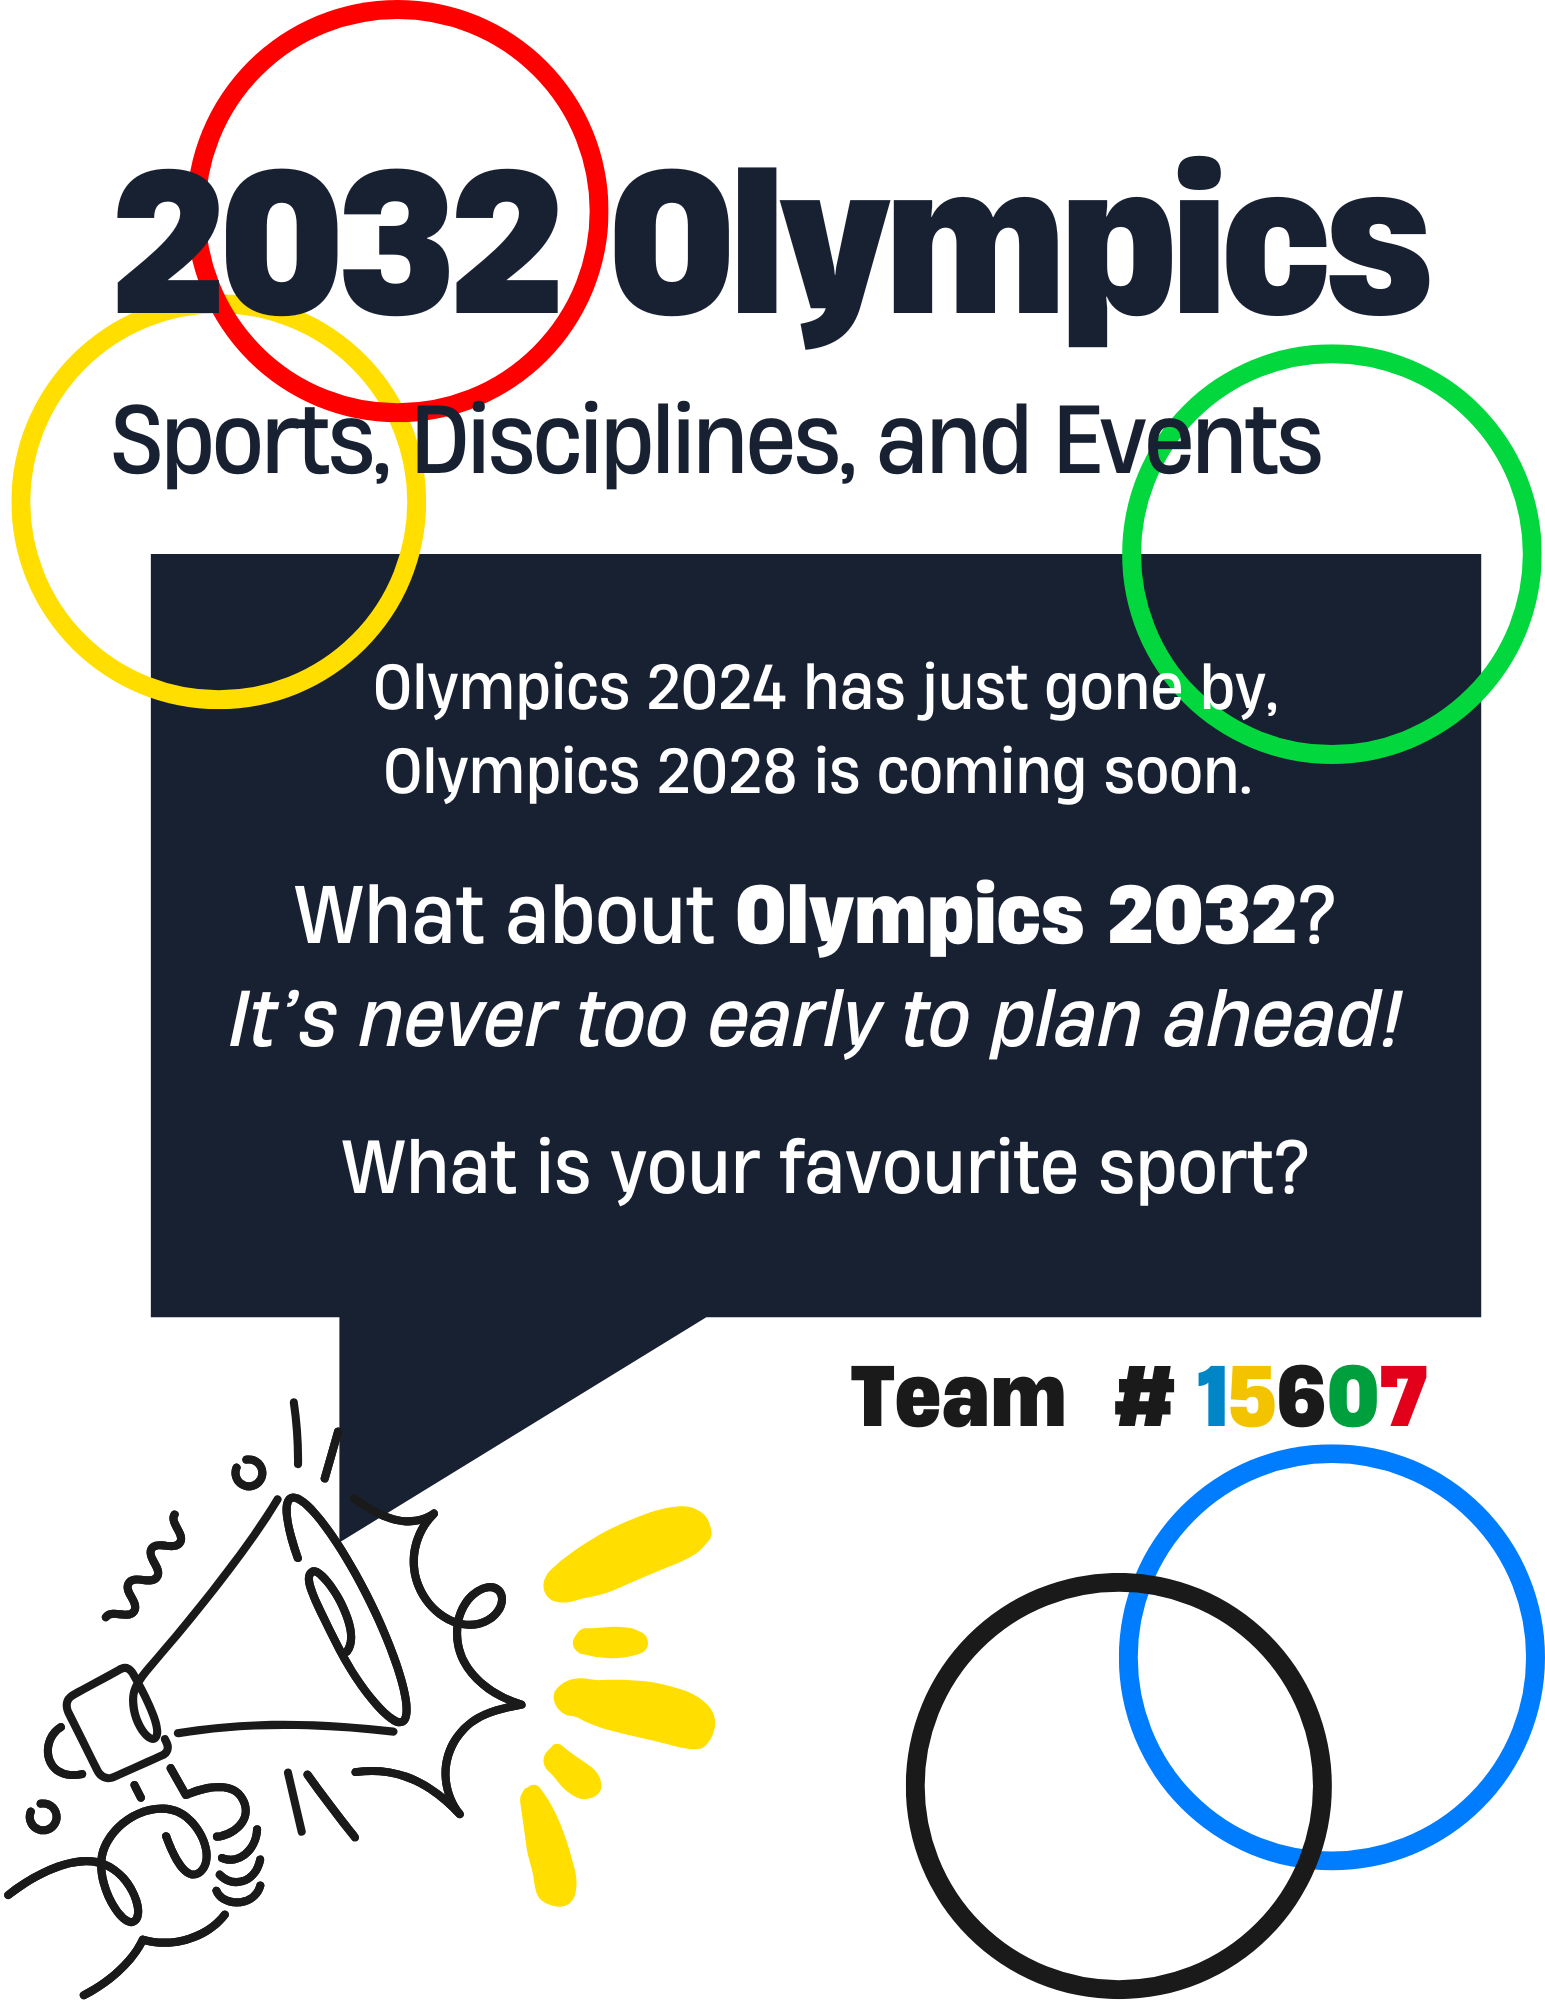
\includegraphics[width=\textwidth, height=\textheight, keepaspectratio]{Olympic.png}

\newpage % 再换页回到正常内容

\tableofcontents


\section{Introduction}

\subsection{Background}

The Olympic Games are a global celebration of friendship, unity, and the pursuit of human excellence. Every four years, athletes from around the world compete under their national flags, inspiring joy and admiration through their skills and determination. From swimming lanes to ice rinks to grassy fields, the Games unite people across continents and cultures.

Each edition of the Games reflects the joint efforts of the host country and the International Olympic Committee (IOC) to deliver an exceptional experience, including the careful selection of sports, disciplines, and events (SDEs).Recent years have seen host nations experiment with SDEs, introducing and removing events during Tokyo 2020, Paris 2024, and Los Angeles 2028. These decisions, made with multiple factors in mind, will shape the Brisbane 2032 Games as well.

To support the Olympic Games in representing their values, our team developed mathematical modesl to provide informed reccomendations for the Brisbane 2032 Games.

\begin{comment}The IOC’s objectives include enhancing global appeal, promoting inclusivity across nations, cultures, and genders, and ensuring fairness, safety, and sustainability. To support these goals, our team is developing mathematical models using comprehensive data. By evaluating SDEs on criteria such as popularity, accessibility, innovation, safety, inclusivity, gender equity, and sustainability, we aim to provide informed recommendations for the Brisbane 2032 Games.\end{comment}

\begin{comment}\textbf{Question 1}: Describe Your Factors 
Find, describe, and justify factors that need to be taken into consideration when fulfilling the IOC criteria. Categorize the factors as quantitative or qualitative, constant or variable, and deterministic or probabilistic. How do these factors affect the Games?

\textbf{Question 2}: Build Your Model
Use the factors outlined in step 1 to build a mathematical model that accurately evaluates SDEs against the Olympic criteria and finds out which SDEs adhere closest to the Olympic standards.

\textbf{Question 3}: Test Your Model
Choose at least three SDEs that have been added or removed from the 2020, 2024, or 2028 games to be evaluated by the model. Do the same for at least three SDEs that have been included in the Games consistently since 1988. Identify similarities and trends between the results of the model and the SDE's current status; discuss how the model explains the SDE's status. Is the model accurate and does it coincide with reality?

\textbf{Question 4}: Rank Potential Additions/Reintroductions
Recommend three SDEs to add to the 2032 Brisbane Games and give each a rank. What SDEs could potentially be included in the Olympics in the far future beyond 2036?

\textbf{Question 5}: Perform A Sensitivity Analysis
Conduct a sensitivity analysis of the model, discuss how it functions and how the factors in step 1 interact with each other: what makes an SDE score well and what makes it score less? Does this make the model more or less realistic? Identify strengths and weaknesses of its decision making.

\textbf{Question 6}: Write A Recommendation Letter
Outline the reasoning for the model and the constructing process in a letter to the IOC. Make suggestions as to which SDEs to add and which to remove; include the results of the SDEs that were evaluated and show how these affect the recommendations. \end{comment}

\subsection{Problem Anaylsis}

The main problem is to develop and refine a mathematical model that quantitatively assesses SDEs against the criteria described by the IOC so that reasonable and logical suggestions can be made regarding the agenda of SDEs that are to be competed at the 2032 Games.Below are the 6 steps to solving the problem.

\textbf{Question 1}: 
To find factors that would affect a SDE’s eligibility in the Olympic Games, our team converted the criteria provided by the IOC into 6 variables. We assess the importance of these variables against each other using the AHP matrix to produce a weight for each of them.

\textbf{Question 2}: 
Our team must create a mathematical model that is able to process individual data from each SDE and convert it into a score after assessing it against the influencing factors. Our team has chosen to use sophisticated models such as AHP, TOPSIS, and the Entropy Method to calculate the weight of each factor and to score our chosen SDEs. When calculated, the comprehensive score encompasses all factors, which have predetermined weights.The SDE with the highest score would be the one that aligns to the IOC’s criteria the most. 

\textbf{Question 3}: 
Using the Olympic Data sheet provided, our team selected a diverse array of Olympic SDEs to be evaluated by our model. This includes SDEs that have attendances that are both consistent and occasional. To test these SDEs against the criteria using our model, we collect data from reliable sources in all aspects of the SDE that are relevant to our factors. Slightly different calculation methods are used to determine the score of each factor. After inputting the data and using our model to output a score for each SDE, we consider their actual Olympic status (consistent or not) and compare our result to it. SDEs with different Olympic statuses should technically be scored differently by our model. We use these tests to evaluate our model’s applicability.

\textbf{Question 4}: 
By our model, we will choose three SDEs that are both not currently in the Olypmics agenda but aligns with the criteria regardless.

\textbf{Question 5}: 
In order to confirm that our model is reliable, we performed a sensitivity analysis on our model. Our team will use this information to discuss what this reveals about the accuracy and reliability of our model. We will also lay out our model’s strengths and weaknesses.

\textbf{Question 6}: 
To convey our ideas and findings, we will adress a letter to the IOC that includes our understanding and general approach to the problem, as well as what we found out after evaluating the SDEs. Within the letter we will make some suggestions as to the addition and removal of some SDEs for the 2032 Brisbane Games, and justify them based on real-world data and the calculations of our model.



\section{Assumptions and Justifications}
\textbf{Here are some additional assumptions that could be made to avoid misunderstandings when evaluating sports against the IOC criteria:}

\begin{comment}\textbf{Assumption 1}: The general injury rate of a sport played by the public is adequate to that when played in the Olympic Games. For the sports that have not yet appeared on the Olympics, we use the general injury rate of that sport to substitutely to rate its safety.
\end{comment}
 
\textbf{Assumption 1}: Anti-doping policies should effectively prevent athletes from taking dopes and other stimulants. The Olympics should have knowledge in both detecting the doping used and preventing the use of stimulated drugs in advance to the game. 

\textbf{Assumption 2}: The popularity and accessibility of a sport are consistent across global regions. We assume that the data on global participation rates and viewership represent a fair average of the sport’s appeal worldwide, without significant regional biases affecting the results.
 
\textbf{Assumption 3}: Sustainability metrics for current Olympic sports apply to future sports under similar conditions. Environmental impact data, such as energy usage and waste management, is assumed to be transferable from current events to proposed new sports, assuming comparable event scales and infrastructure.
 
\textbf{Assumption 4}: The number of participating countries is a reliable measure of inclusivity.  We assume that the number of nations actively engaging in a sport indicates its accessibility and cultural relevance, regardless of variations in the level of competition or infrastructure availability in those countries.
 
\begin{comment}\textbf{Assumption 5}: Sports designed for younger audiences can maintain appeal over time. We assume that the inclusion of sports like Breaking or Skateboarding aligns with long-term trends rather than short-term fads, ensuring continued relevance and innovation.\end{comment}
 
\textbf{Assumption 5}: Gender equity assessments are based on current participation and event structures.  We assume that any gender imbalances in participation or event availability reflect existing limitations rather than deliberate exclusion, and that these can be addressed through structural adjustments in the future.
 
\textbf{Assumption 6}: Safety and injury rates account for Olympic-level training and standards.  Injury rates are assumed to reflect conditions where athletes receive optimal training, equipment, and medical care, as is standard in the Olympics, making general public injury rates a conservative estimate for comparison.
 
\begin{comment}\textbf{Assumption 8}: Data sources are accurate, reliable, and representative.  We assume that the datasets used for participation, injury rates, sustainability, and other factors are up-to-date and representative of the sport’s current state, avoiding significant inaccuracies.\end{comment}
 
\textbf{Assumption 7}: The total number of participating NOCs in future Olympic Games will stay constant over time. It is assumed that there will be no major, unpredictable fluctuations in the number of NOCs that participate in the Olympic Games; that is, the total number of participating NOCs in the Paris 2024 Games serves as an accurate representation of future Games.

\section{Variables}



    \begin{figure}[H]
    \centering
    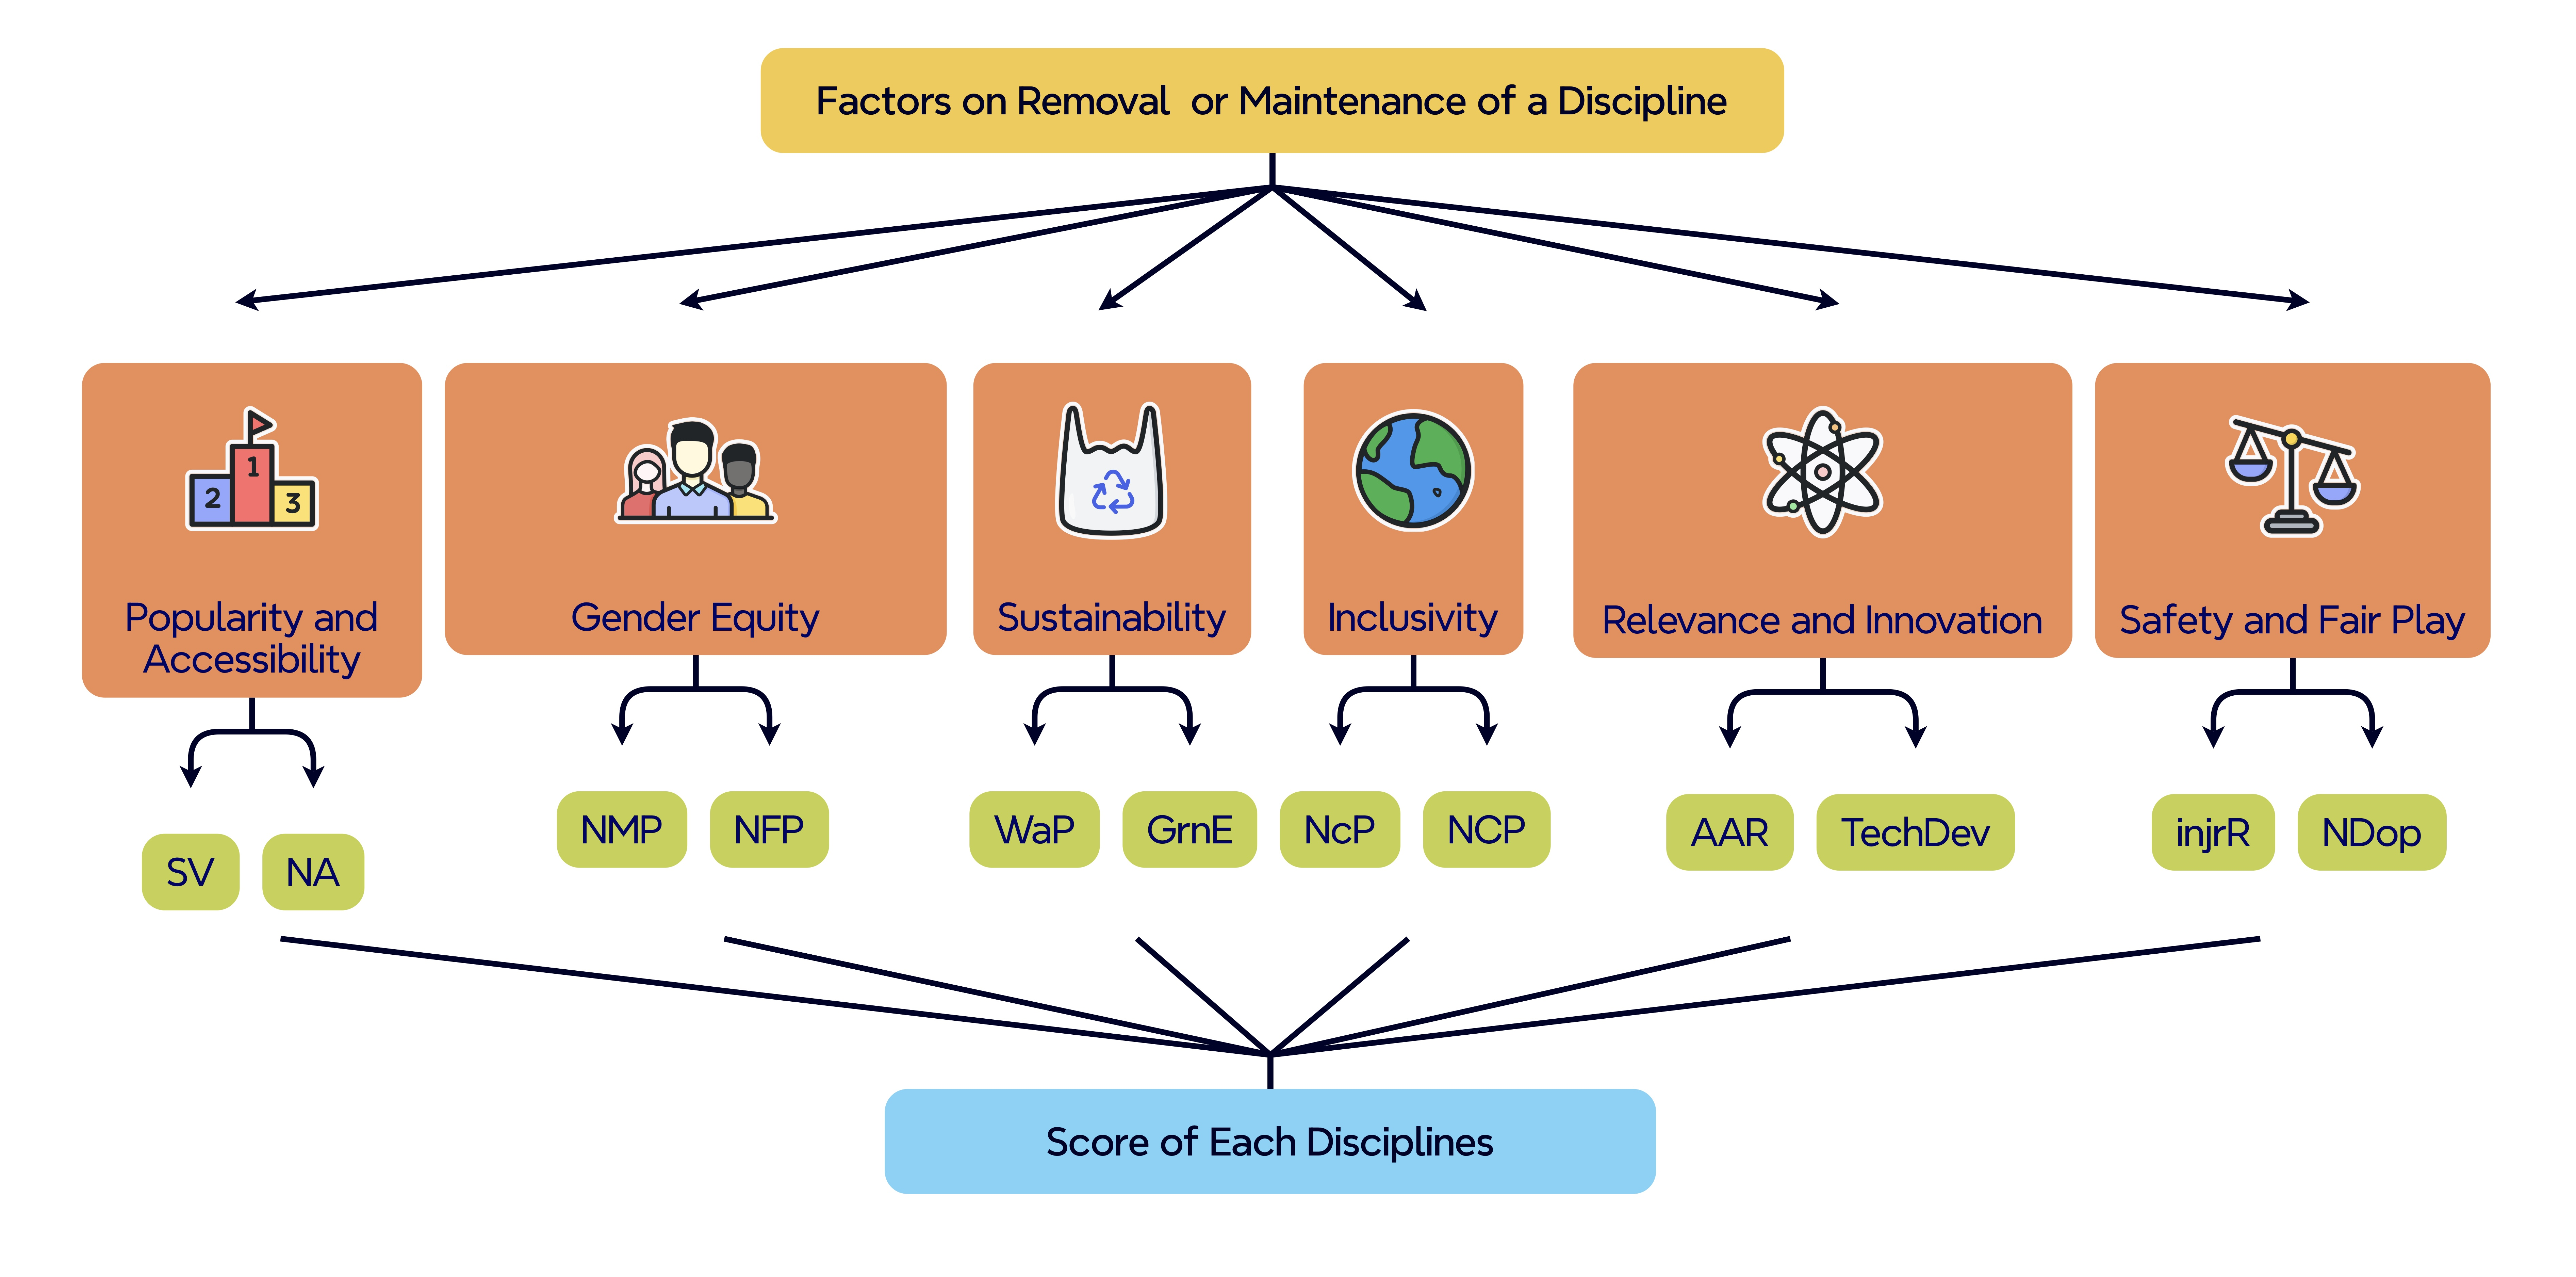
\includegraphics[width=1\textwidth]{Factor.png}
    \caption{\label{fig:Factor} }
    
\end{figure}
In the process of considering different sports, disciplines, and events (SDEs) for either addition or removal from the 2032 Summer Olympic Games, a variety of factors come into play. Our factors have taken into account the criteria provided by the IOC’s Olympic Programme Commission. To provide a clear picture of each factor we have incorporated into our model, we have listed each factor below and their categorization of quantitative/qualitative, variable/constant, and deterministic/probabilistic.

\begin{table}[H] % Add [H] here to force placement
    \centering
    \begin{tabular}{c|c}
      NMP & Number of Male Participants \\
      NFP & Number of Female Participants \\
      SV & Search Volume \\
      NA & Number of Audience \\
      WaP & Waste and Pollution \\
      GrnE & Green Energy \\
      NCP & Number pf Continent Participated \\
      NcP & Number of Country Participated \\
      AAR & Audience Age Range \\
      TechDev & Technology Development \\
      injrR & Injure Rate \\
      NDop & Number of Doping \\
    \end{tabular}
    \caption{Variables Name and Meaning}
    \label{tab:my_label}
\end{table}

\section{Model Overview}
    \begin{figure}[H]
    \centering
    \includegraphics[width=1\textwidth, height=7.5cm]{Introduce.png}
    \caption{\label{fig:Introduce} }
\end{figure}
\subsection{Analytical Hierarchy Process (AHP)}
The analytical Hierarchy Process is a mathematical model used to analyze the system of complex decisions based on mathematics and psychology. It quantifies the weights of each factor influencing the decision-making by comparing the importance between each pair of factors depending on individuals’ experiences. 
The first step in AHP model is to come up with a Pair-wise comparison matrix, where all factors are aligned by a hierarchical model:


\[
A = 
\begin{bmatrix}
    1 & a_{12} & a_{13} & \cdots & a_{1n} \\
    \frac{1}{a_{12}} & 1 & a_{23} & \cdots & a_{2n} \\
    \frac{1}{a_{13}} & \frac{1}{a_{23}} & 1 & \cdots & a_{3n} \\
    \vdots & \vdots & \vdots & \ddots & \vdots \\
    \frac{1}{a_{1n}} & \frac{1}{a_{2n}} & \frac{1}{a_{3n}} & \cdots & 1
\end{bmatrix}
\]

Where \(a_{ij}\) expresses that level of importance of \(i\) compared to j, and \(a_{ij}=1\) when \(i=j\). And with a given value \(a_{ij}=v\), the value of its reciprocal is double obtainable, where \(a_{ij}=\frac{1}{v}\). We then assign values to the matrix by comparing the importance of each group of pair-wise groups according to the following scale:

\begin{table}[ht]
    \centering
    \begin{tabular}{@{}llp{10cm}@{}}
        \toprule
                 &\textbf{Definition} & \textbf{Explanation} \\ 
        \midrule
        1 & \textbf{Equally Preferred} & Two activities contribute equally to the objective. \\
        3 & \textbf{Moderately Important} & Experience and judgment slightly favor one activity over another. \\
        5 & \textbf{Strong Importance} & Experience and judgment strongly or essentially favor one activity over another. \\
        7 & \textbf{Noticeable Dominance} & An activity is strongly favored over another, and its dominance is demonstrated in practice. \\
        9 & \textbf{Extreme Importance} & The evidence favoring one activity over another is of the highest degree possible of affirmation. \\
        2,4,6,8 & \textbf{Intermediate Values} & Used to represent compromise between the preferences listed above. \\
        \bottomrule
    \end{tabular}
    \caption{AHP Pairwise Comparison Scale}
    \label{tab:ahp_scale}
\end{table}

The weight of each factor in the group can be calculated as below:
\[
p_{i}=\frac{1}{n}\sum_{m=1}^{n}a_{im}
\] 
 However, with the matrix filled out, the values within the matrix may not be consistent, as the values are being judge independently in pairs without considering the clustered relationships in groups(e.x. \[a_{13}\neq a_{12} \cdot a_{23}\]. Therefore, the final step is to check the consistency of the model. To do this, AHP calculates the consistency ratio (CR), the consistency index (CI), and the random-like matrix (RI). These can be defined as:
 \[
 CI=\frac{\lambda-n}{n-1}
 \]
 \[
 RI=\sum_{m=1}^{n}\frac{CI_{m}}{n}
 \]
 \[
 CR=\frac{CI}{RI}
 \]
 The consistency ratio, when lesser or equal to 0.1, determines the AHP analysis is acceptable to be continued on. 
\begin{figure}[H]
    \centering
    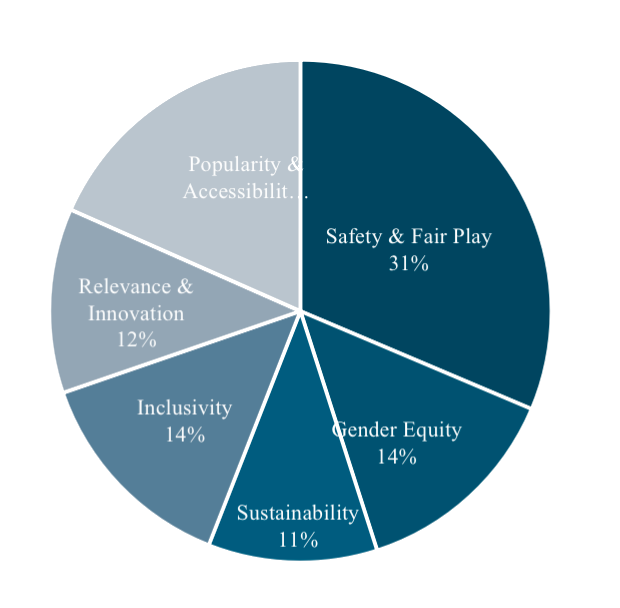
\includegraphics[width=0.5\textwidth]{pigraph (1).png}
    \caption{\label{fig:pigraph} }
\end{figure}
 The final weight we arrived at after applying the APH analysis is as follows.

\subsection {Technique for Order Preference by Similarity to Ideal Solution (TOPSIS)}
TOPSIS is a sophisticated and widely-used multi-criteria decision-making technique our team employed to calculate and rank each SDE in regards to its scoring in each of the factors. 

The objective of TOPSIS is to use criteria and data from each of the alternative solutions to determine a fictional ideal solution and an anti-ideal solution. It then calculates the distance from the position of each alternative solution to the ideal solution and the anti-ideal solution. It stands to reason that an optimal solution would have a shorter distance from the ideal solution and a longer distance from the anti-ideal solution. Based on these distances, the algorithm produces a score and a rank for each alternative solution. The score, is labeled the closeness coefficient, with a larger coefficient denoting a more optimal solution and a smaller one, less.
The closeness coefficient is calculated as such:

\[
CC_{j} = \frac{D_{i}^-}{D_{i}^+ + D_{i}^-}
\]
where: 
\begin{itemize}
   \item \( D_{i}^+ = \) Distance of the alternative from the ideal solution.
    \item \(D_{i}-=\) Distance of the alternative from the negative-ideal solution.
\end{itemize}
The closeness coefficients are used to compare against one another and produce a rank for each alternative solution.

The advantage of TOPSIS is that it mimics human rationale when making decisions—taking into account a multitude of factors and considering if each solution is nearer to an ideal.

In the case of assessing potential Olympic SDEs against the IOC’s criteria and our team’s factors, each SDE would represent an alternative solution. The ideal solution would be a combination of the highest factor scores out of all the SDEs while the anti-ideal solution would be a combination of the lowest factor scores. The analysis will measure the distance each SDE has from the “ideal SDE” and from the “anti-ideal SDE”, producing results as described above. 
TOPSIS itself is presented and functions as a software program. Our team can run code programs to complete our TOPSIS analysis of each SDE.
TOPSIS is helpful in the solution of our problem because it gives a mathematically accurate assessment of the SDEs using the factor scores we devised.

\subsection{Entropy Method}
To address the subjectivity of the AHP method, which relies on pairwise comparisons based on subjective judgments, we introduced the Entropy Weight Method (EWM). EWM, a data-driven approach rooted in information theory, objectively assigns weights by analyzing the information distribution within the dataset.





By combining AHP's structured subjectivity with EWM's objectivity, this hybrid approach achieves a balanced and reliable framework for evaluating factors such as popularity, sustainability, gender equity, and innovation. This ensures a more robust decision-making process, reducing bias while leveraging both human expertise and data insights.

\begin{itemize}
   \item \textbf{Proportion Matrix Calculation:} 
\[
    p_{ij} = \frac{x_{ij}}{\sum_{i=1}^{n} x_{ij}}
\]
where \(x_{ij}\) represents the value of project \(i\) for factor \(j\), and \(\sum_{i=1}^{n} x_{ij}\) is the total for factor \(j\).

    \item \textbf{Entropy Calculation:}
\[
e_{j}=-k\sum_{i=1}^{n} p_{ij}ln(p_{ij}) , k = \frac{1}{ln(n)}
\]

where \(n\) is the number of projects, and \(p_{ij}ln(p_{ij})\) is defined as 0 when \(p_{ij}=0\)

    \item \textbf{Redundancy Calculation:}
\[
d_{j}=1-e_{j}
\]

Redundancy reflects the information utility of each factor

    \item \textbf{Weight Determination:}

\[
w_{j}=\frac{d_{j}}{\sum_{j=1}^{m}}d_{j}
\]
\end{itemize}

To integrate the results of the Analytical Hierarchy Process (AHP) and the Entropy Weight Method(EWM), we utilize the \textbf{geometric mean} to balance subjective judgments with data-driven objectivity By using element-wise multiplication, the multiplicative method emphasizes the alignment between subjective judgments and objective data.

Given the weights \(w_{j}^{AHP}\) from the AHP model and \(w_{j}^{Entropy}\) from the Entropy method, the combined weight \(W_{j}\) for factor \(j\) is calculated as: 

\[
W_{j}=\frac{
\sqrt{w_{j}^{AHP}\cdot w_{j}^{Entropy}}
}
{
\sum_{j=1}^{m}\sqrt{w_{j}^{AHP}\cdot w_{j}^{Entropy}}
}
\]

where: 

\begin{itemize}
    \item \(w_{j}^{AHP}\cdot w_{j}^{Entropy}\) represents the element-wise multiplication of weights from the two methods

    \item \(\sum_{j=1}^{m}w_{j}^{AHP}\cdot w_{j}^{Entropy}\) normalizes the combined weights so that their total sums to \(1\)
    
    \item m is the total number of factors
\end{itemize}


The geometric mean highlights the agreement between AHP and entropy weights, ensuring factors that score high in both methods are emphasized while minimizing the impact of outliers.



\section{Variables Indexes}
\textbf{{Popularity and Accessibility}}

{Introduction to Popularity and Accessibility}

\textbf{Popularity and Accessibility} are key criteria for evaluating the suitability of sports disciplines for the Olympic Games. Popularity reflects global interest and engagement, encompassing both offline audience size and online metrics, such as social media activity and streaming views. Accessibility, on the other hand, focuses on the practical feasibility of hosting a sport, with venue costs being a major consideration. These two factors are closely intertwined—greater promotion can increase popularity, but it might also drive up costs, leading to higher ticket prices and potentially limiting audience reach.

A balanced approach is essential when assessing sports disciplines. Popularity should take into account both digital engagement and live audience response, while Accessibility can be evaluated through venue-related costs and infrastructure requirements. This dual framework ensures that chosen sports not only captivate global audiences but also remain financially viable, aligning with the International Olympic Committee’s goal of maximizing appeal while minimizing barriers.
\textbf{Methodology}
To ensure a balanced evaluation, our methodology integrates various data points to capture both the popularity and feasibility aspects of Olympic sports. This method integrates online data (e.g., Google Trends), offline audience data, and venue costs to provide a holistic view of each sport's appeal and practical viability.

\textbf{Data Sources and Variables}
\begin{comment}To thoroughly evaluate the popularity and accessibility of Olympic sports, we utilized three primary data sources: online search trends, offline audience attendance, and venue costs. Each dataset provided a unique lens through which we could understand a sport's appeal and logistical feasibility.\end{comment}

\begin{enumerate}
    \item \textbf{Google Trends Data}
    Google Trends was chosen to measure online popularity, reflecting global interest in each sport. Using a Python-based tool, we retrieved search interest scores from 2014 to 2024.
    \begin{itemize}
    \item \textbf{Keyword Selection:}
     To ensure comprehensive representation, multiple keywords were analyzed for each sport. For example:
         \begin{itemize}
             \item \textbf{Swimming:} “Swimming,” “Freestyle Swimming,” “Butterfly Swimming.”
             \item \textbf{Athletics:} “Track and Field,” “Marathon,” “Sprinting.” 
         \end{itemize}
    \end{itemize}

    The average score across all relevant keywords provided a reliable metric for assessing online engagement.
    \begin{figure}[]
        \centering
        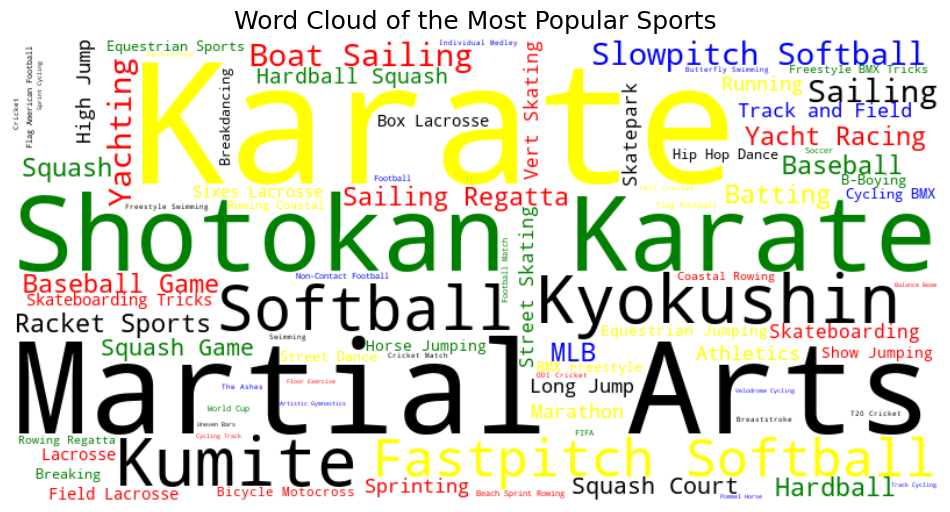
\includegraphics[width=0.8\textwidth]{Word Cloud.png}
        \caption{Word Cloud - Keyword Analysis \label{fig:Word Cloud}}
    \end{figure}

    \item \textbf{Offline Audience Attendance}
    We estimated offline popularity based on historical data from recent Olympic venues.
    \begin{itemize}
        \item \textbf{Venue Capacity:} For instance, the Tokyo National Stadium (68,000 seats for athletics) and the Tokyo Aquatics Centre (15,000 seats for swimming).
        \item \textbf{Occupancy Rates:} These ranged from 70\% to 90\%, depending on each sport's historical trend.
        \item \textbf{Example:} For athletics, with a 90\% occupancy rate, estimated attendance was \(68,000 \cdot 0.90=61,200\).
    \end{itemize}
    \item \textbf{Venue Costs (Accessibility)} 
    Venue costs included construction, maintenance, and operational expenses, derived from IOC reports. Accessibility scores were calculated using this formula:
    \[
    Accessibility = 1 - Normalized \cdot Cost
    \]
    Higher venue costs resulted in lower Accessibility scores, reflecting the inverse relationship between cost and feasibility.
\end{enumerate}
\textbf{Composite Scoring}
This section explains the process of integrating normalized metrics for Google Trends (online popularity), offline audience attendance, and venue costs (accessibility) into a unified composite scoring framework. The methodology balances audience engagement with logistical feasibility to evaluate the relative suitability of sports disciplines for the Olympic Games.
\textbf{Scoring Formula}
The composite score was computed as a weighted combination of three normalized metrics:

Composite Score \(=w_{1} \cdot GoogleTrends_Norm + w_{2} \cdot Attendance_Norm + w_{3} \cdot Accessibility\)


Where:
\begin{itemize}
    \item \(w_{1}=0.4\): Weight for Google Trends data, representing online popularity
    \item \(w_{2}=0.4\): Weight for audience attendance, capturing offline popularity.
    \item \(w_{3}=0.2\): Weight for accessibility, derived from venue costs.
\end{itemize}
The weight distribution reflects the importance of audience engagement (online and offline) over logistical feasibility, in alignment with the IOC’s priorities.

\textbf{Data Processing}
\begin{enumerate}
    \item \textbf{Normalization:}
    To ensure comparability across different metrics, all data were normalized using Min-Max scaling:
    \[
    X_{\text{Norm}} = \frac{X - X_{\text{Min}}}{X_{\text{Max}} - X_{\text{Min}}}
    \]
    \begin{itemize}
        \item \textbf{GoogleTrends\_Norm:} Normalized global search interest data, reflecting online popularity.
        \item \textbf{Attendance\_Norm:} Normalized audience attendance, representing offline engagement.
        \item \textbf{Cost\_Norm:} Normalized venue costs, used to calculate accessibility.
    \end{itemize}

    \item \textbf{Accessibility Calculation:}
    Accessibility was calculated as the inverse of normalized venue costs:
    \[
    \text{Accessibility} = 1 - \text{Cost\_Norm}
    \]
    This ensures that sports with higher venue costs are assigned lower accessibility scores, emphasizing the feasibility of hosting.

    \item \textbf{Composite Score Calculation:}
    Each sport’s composite score was derived by applying the weights to the normalized metrics. The resulting scores were ranked in descending order to identify the top-performing sports.
\end{enumerate}

\textbf{Results}
After applying Min-Max normalization to Google Trends data, audience attendance, and venue costs, a composite score was calculated for each sport. These scores provide a unified evaluation of each discipline's popularity and accessibility, with higher scores indicating better suitability for the Olympics.

The bar chart below illustrates the composite scores for all sports disciplines, sorted from highest to lowest. The chart highlights the relative strengths and weaknesses of each sport in terms of online popularity, offline engagement, and accessibility.

\textbf{Model Results}

\textbf{Gender Equity}
Gender Equity is a cornerstone of the Olympic Games, reflecting the values of inclusivity, fairness, and equal opportunity. Ensuring balanced representation for both male and female athletes fosters a more diverse and globally resonant event. Gender equity also contributes to the integrity and sustainability of the Olympics by promoting a fair distribution of opportunities and reinforces the ethical commitment of the Games to fairness and diversity. In our model, we assess gender equity by analyzing the proportion of male and female participants in each SDE and the availability of events for both genders. SDEs that demonstrate clear gender imbalances are less aligned with Olympic values and thus rated less favorably in this criterion.
To evaluate the gender equity of each sport, we use an index calculated as
\[\frac{|NMP-NFP|}{NMP+NFP}\]
This index provides a measure of the balance in male and female participation, with values closer to zero indicating greater gender equity. For sports that have already been included in the Olympics, we obtain the number of male and female participants from the most recent Olympic Games. For disciplines that have not yet been featured in the Olympics, we source participation data from international events organized by the sport’s governing body. This approach ensures that our evaluation is based on the most relevant and up-to-date data available, allowing for consistent comparisons across all sports and disciplines.

\textbf{Sustainability}
Sustainability is a critical factor in evaluating Olympic sports. For our model, we considered three key areas: environmental impact, infrastructure costs, and sustainability initiatives. Each factor was assigned a different weight based on its significance.

The cost of infrastructure is a major consideration, so we assigned this factor the highest weighting of 40%. \begin{comment}Some sports require extensive new facilities, while others rely on existing venues. Higher infrastructure costs often correlate with greater environmental impacts, such as pollution, habitat loss, and landfill waste. For this reason, we assigned this factor the highest weighting of 40%.\end{comment}

The environmental impact of a sport reflects how eco-friendly its operations are. Sports that utilize green energy, reduce pollution, and minimize damage to the environment score higher. For example, skateboarding at the Paris Olympics used temporary setups to avoid new construction, while Stade de France, hosting athletics, operates on renewable energy with sustainable transport options. Environmental impact is weighted at 30%.
Lastly, sustainability measures how a sport promotes initiatives like reuse, eco-friendly designs, and habitat protection. Sports with higher scores positively influence global audiences. For instance, sailing at the Paris Olympics emphasized marine protection, while squash, planned for the 2028 Games, scored lower due to its lack of environmental initiatives. Sustainability carries a weighting of 30%.

\textbf{Inclusivity}
One of the IOC’s criteria is that each SDE must be inclusive and representative of diverse cultures and countries and that at least 75 countries should practice this sport. A SDE that only a minority of countries practice would serve against Olympic standards as is less representative of universal civilization as a whole and lessens global participation. In our model, we calculate an SDE’s inclusivity by dividing the number of participating National Olympic Committees (NOCs) in the SDE by the total number of participating NOCs in the Paris 2024 Games. For SDEs that did not compete in the Paris 2024 Games, we replaced the numerator with the number of countries that participated in the most recent world competition of that SDE. It should be noted that the number of continents participated in the events and Olympics of all SDEs is 5, which is the maximum amount. Since all SDEs satisfy the maximum number of continents, this variable has been omitted within the score calculation of the inclusivity factor to measure the actual difference between the SDEs.

The score of the inclusivity factor is then normalized by setting the highest data point out of the SDEs chosen as a score of 100, and the lowest as a score of 0. An SDE with a higher score is considered more inclusive and increases its overall accordance with the IOC’s criteria.

\textbf{Relevance and Innovation}
Relevance and innovation are crucial in assessing Olympic sports, focusing on modern trends, youth engagement, and technological integration. To evaluate this, we analyzed AI Usage, Maximum Tickets for Each Venue, Primary Viewers, and Demographics, with weights reflecting their impact.
AI Usage (30\%) considers a sport’s technological integration. Gymnastics and athletics scored highly for innovations like AI-enhanced judging, while sports like lacrosse scored lower.
Maximum Tickets for Each Venue (25\%) reflect audience size. High-capacity venues like Stade de France for athletics scored well, while smaller sports like squash ranked lower.
Primary Viewers (25%) assesses appeal to younger audiences. Youth-driven sports like skateboarding scored highly, unlike niche sports with limited appeal.
Demographics (20%) measures cultural diversity. Football and cricket, with global reach, scored higher, while sports with localized followings scored lower.
This approach ensures sports remain innovative, widely appealing, and inclusive of Olympic values

\textbf{Safety and Fair Play}
Safety and Fair Play are crucial factors when judging whether a sport resonates with the values of the Olympic games. Athletes' performances are largely dependent on their physical well-being, undermine the value of the Olympic games and seriously distort individual performances. Physical protection and Anti-doping policies play a vital role in guaranteeing the fairness of the game in response to the ethics of the Olympics. Fairness and safety are considered the most important factors in our model.

\textbf{Safety}
To rate the safety of SDE, we consider the official injury rate of sports in the Olympic games. SDE with the highest injury rate receives 0 on the safety section, whereas that with the lowest injury rate receives 100. Safety is weighted 50% of the importance in Safety and Fair Play. 

\textbf{Fair Play}
The number of detected doping cases in an Olympic sport is used to rate the fairness of the game. However, if the sport hasn't appeared in the Olympics before, this part of the criteria will be neglected and its score will be totally dependent on the safety score.

\section{Testing the Model on 14 Olympic Sports}
\subsection{Results and Analysis}
\begin{figure}[H]
    \centering
    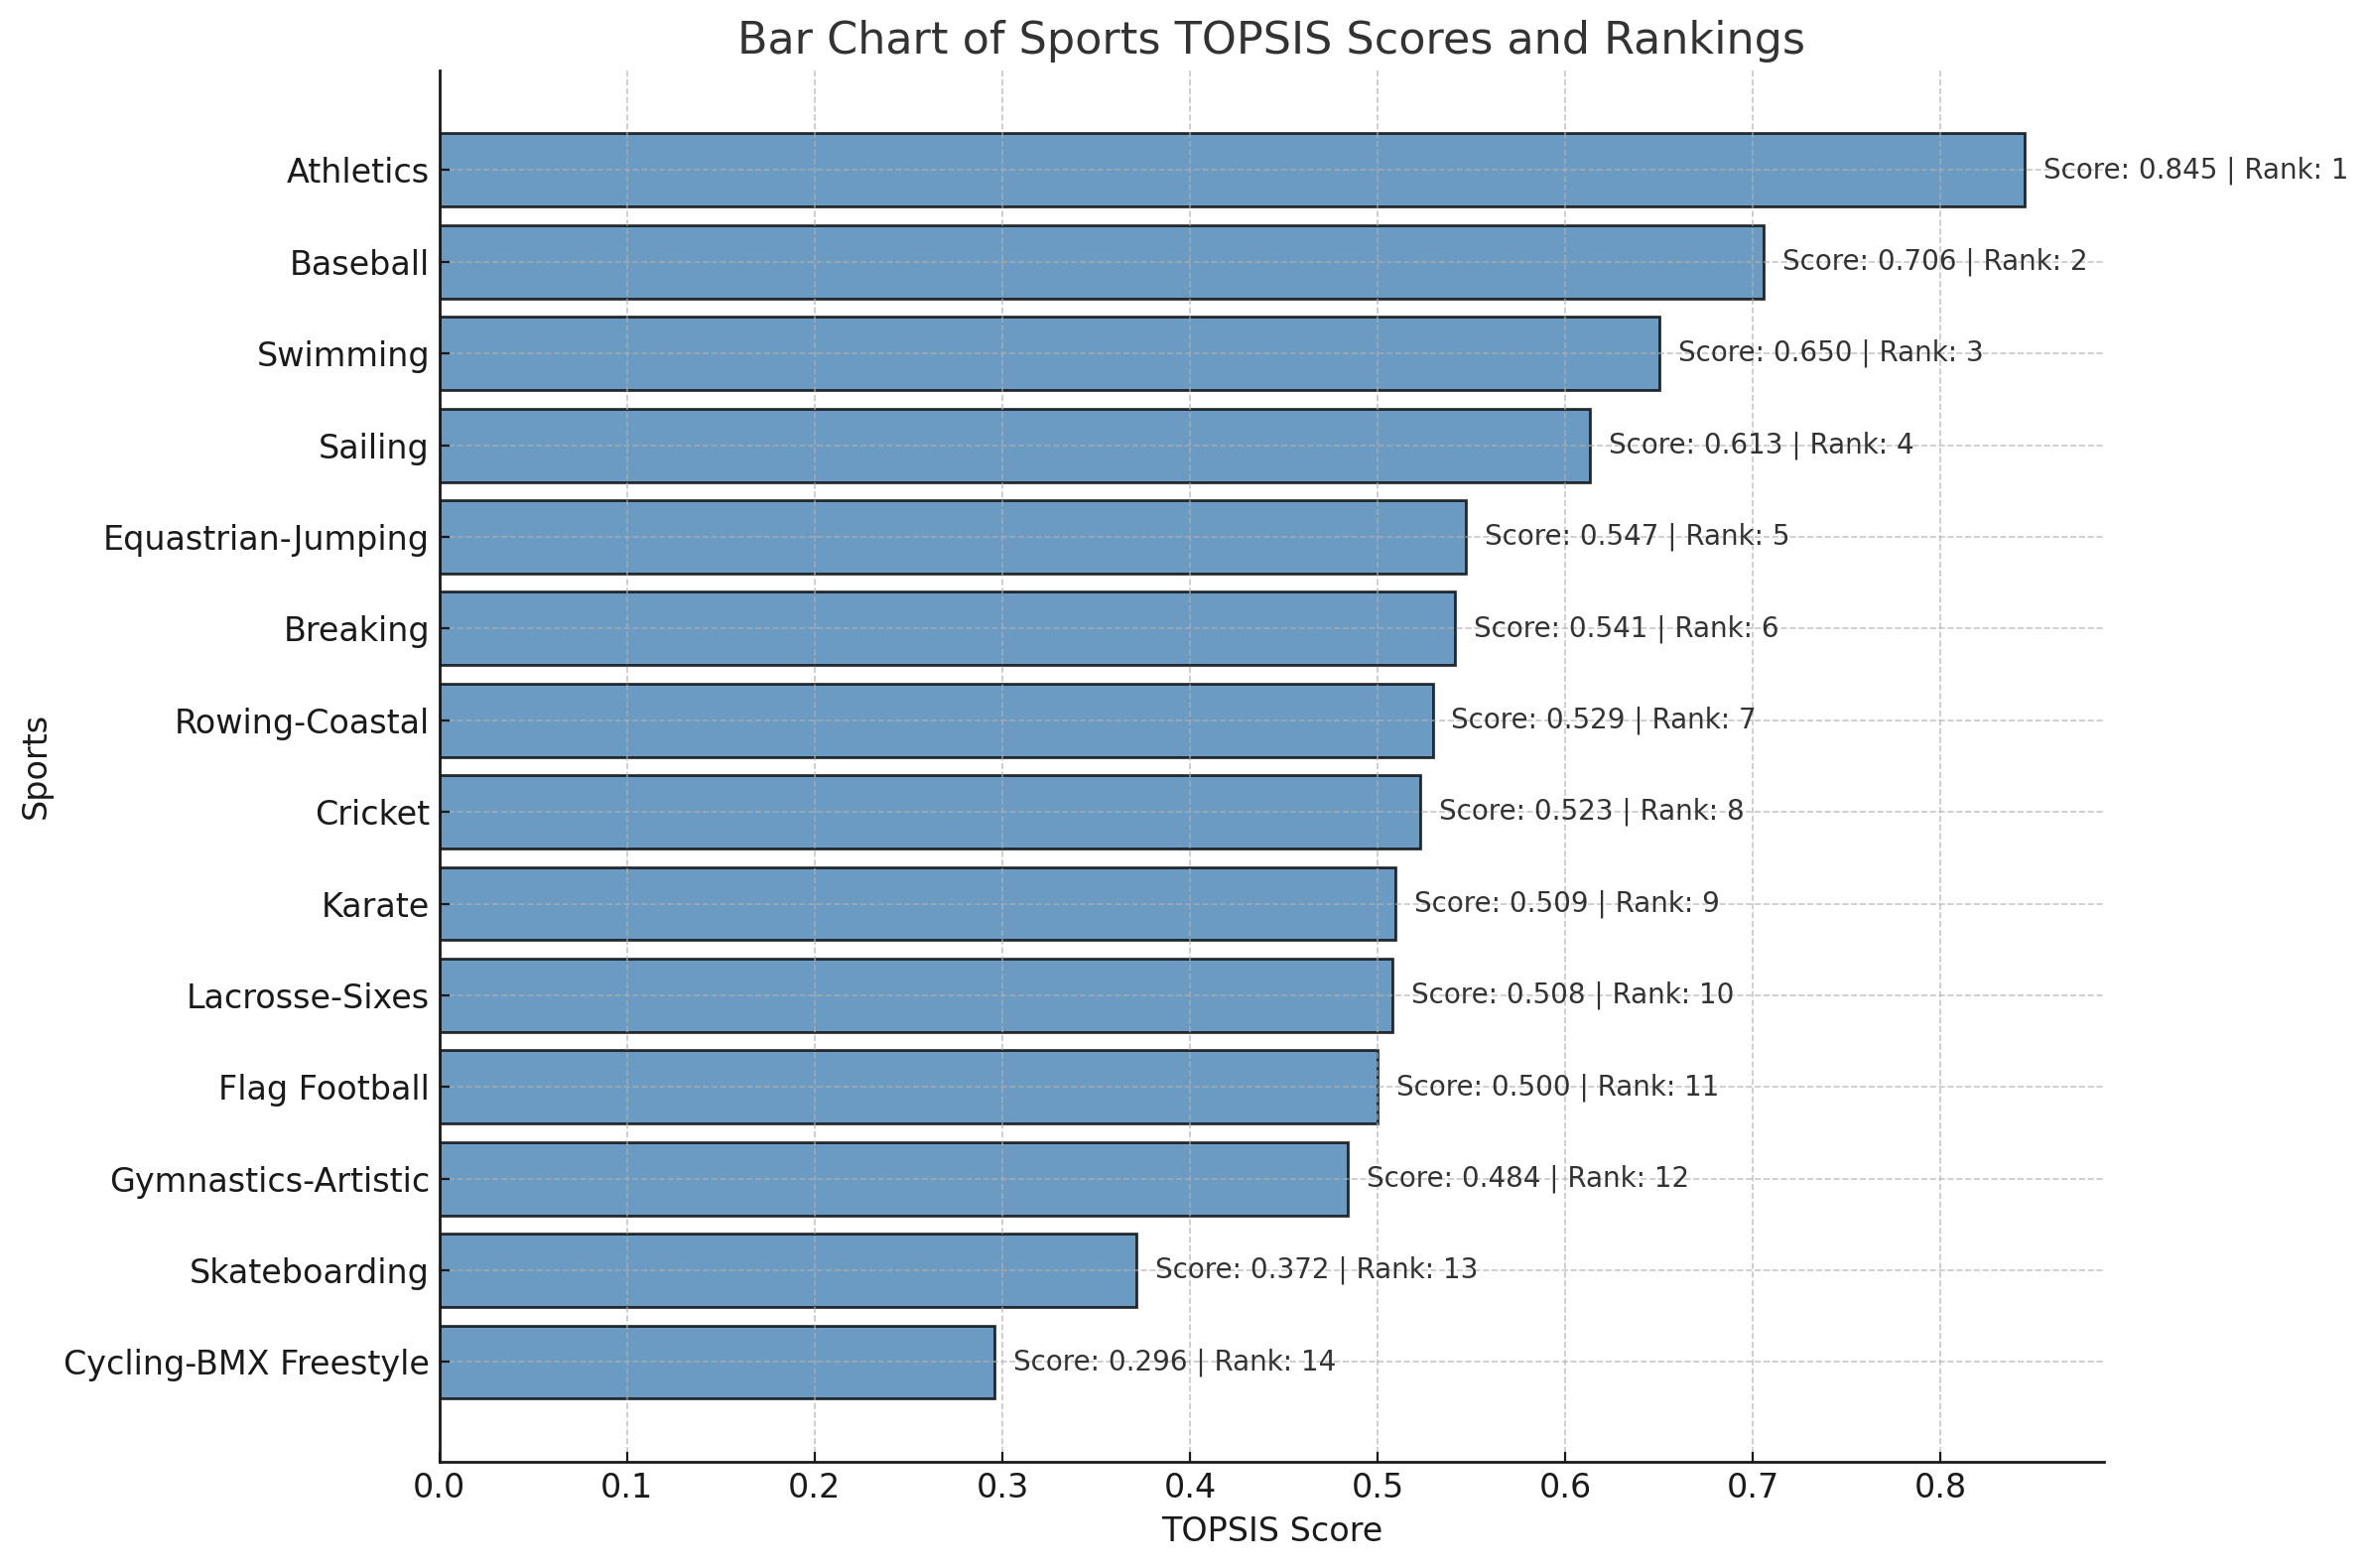
\includegraphics[width=1\textwidth]{bargraph.jpg}
    \caption{\label{fig:}}
\end{figure}
We organized the TOPSIS score of the 14 tested SDEs into the graph below. This can show the extent to which each sport displays Olympic values and ethnics. By comparing the result of our model to the actual Olympic data, we want to show the reliability of our model in evaluating the relevance of Olympic sports.

\subsubsection{SDEs continuously been in the Olympic Programme since 1988:}

\textbf{Swimming} is ranked \textbf{3rd} in the model. In reality, swimming has been a prominent SDE (Sport, Discipline, Event) in the Olympics since 1896, with more than 30 swimming events each year since 1988. This long-standing role in the Olympic Games corroborates with the model's ranking.

\textbf{Athletics}, ranked \textbf{1st} in the model, has had more than 41 events each year in the Olympics since 1988. This substantial number of events highlights athletics' even more prominent role in the Olympics compared to swimming, aligning well with the model’s ranking.

\textbf{Baseball} is ranked \textbf{2nd} in the model. However, compared to its high ranking in our model, the number of baseball events appeared intermittently only after 1992. It have been removed and reintroduced several times between the late 1800s to the early 1900s. This may show inconsistency between our model and the Olympic Games. Baseball, indeed, is a sport that strongly reveals the Olympic's values. This discrepancy may be explained by the prevalence of other major baseball competitions in the world that call off the importance of having another major baseball event. 

\begin{comment}\textbf{Cycling-Track} is ranked \textbf{16th} in the model, one of the lowest rankings. However, cycling has been an Olympic event since 1896, indicating a lack of correlation between the model and the actual Olympic history. The model seems to understate the significance of cycling’s long-standing Olympic presence.\end{comment}

\textbf{Equestrian-Jumping}, ranked \textbf{5th} in the model, has been part of the Olympics since 1912. While the event occurs less frequently each year, it plays an important role in showcasing Olympic ethics. The lower ranking reflects its sparse occurrence rather than its importance in Olympic tradition.

\begin{comment}\textbf{Football} is ranked \textbf{13th} in the model, even though it has been an Olympic sport since 1900. This ranking discrepancy suggests that the model may undervalue football's global presence and historical significance in the Olympics.\end{comment}

\textbf{Gymnastics-Artistic}, ranked \textbf{10th} in the model but has been a constant in the Olympics since 1896. With numerous events each year, the model’s ranking seems to downplay gymnastics' consistent Olympic presence.

\textbf{Sailing}, ranked \textbf{4th} in the model, has been included in the Olympics since 1896, with approximately 10 events each year since 1988. The model’s ranking aligns with sailing’s continuous presence and importance in the Olympics.

\textbf{Conclusion}: Five out of six sports—\textbf{Swimming}, \textbf{Athletics}, \textbf{Equestrian-Jumping},\textbf{Baseball}, and \textbf{Sailing} ranked on the first half of our model, and therefore show a strong correlation with the model. However, the discrepancies between our model and the Olympics data in \textbf{Gymnastic-artistic} indicate that the model still need adjustments to better reflect the actual historical and global significance of these sports in the Olympic Games. Looking closely into the historical social circumstances of each individual SDEs may help improve the performance of our model.

\subsubsection{SDEs being added or removed since 2020:}

\begin{comment}\textbf{Softball} is ranked \textbf{6th} in our model, but it has only had 7 events in the Olympics since 1988. Softball has consistently been added and removed from the Olympic sports list. This sporadic presence indicates that while the sport has a role in the Olympics, its importance is less than other long-standing events, which is reflected in the model’s ranking.\end{comment}

\textbf{Breaking}, ranked \textbf{6th} in our model, will have only 2 events in the 2024 Olympics. Although breaking may represent the Olympic values of youth engagement and global reach, it is insufficiently established compared to other sports and does not yet stand as an important Olympic sport, as confirmed by both the model and the real-world situation.

\textbf{Cricket}, ranked \textbf{8th} in our model, has only appeared in 3 Olympic events. It is not currently seen as an event that compellingly aligns with the values of the Olympics, a conclusion that is echoed by both the model and the real-world data.

\textbf{Cycling-BMX Freestyle} is ranked \textbf{12th}, the lowest in our model. This sport has only been included since the 2020 Olympics with 2 events per year. The model’s ranking is consistent with its limited presence in the Olympics, indicating that BMX freestyle has not yet achieved significant Olympic status.

\textbf{Flag Football} is ranked \textbf{9th} in our model but is only set to debut at the 2028 Olympics. Both the model and the real-world data suggest that flag football has not yet proven itself to be a sport that fully aligns with the IOC's criteria for Olympic inclusion.

\textbf{Karate} is ranked \textbf{7th} in our model. Although it was included in the 2020 Tokyo Olympics with 8 events, it will be removed from the 2024 Olympics. This temporary inclusion, likely driven by the host nation Japan, signals that karate may not have long-term significance in the Olympics, which aligns with its ranking in the model.

\textbf{Lacrosse-Sixes} is ranked \textbf{8th} in our model, with 2 planned events in the 2028 Olympics. The model and real-world data show that lacrosse-sixes does not yet convincingly appeal to the Olympic values and is not expected to play a prominent role in future Olympic Games.

\textbf{Skateboarding}, ranked \textbf{11th} in our model, has had 4 events per year since its inclusion in the 2020 Olympics. While skateboarding has not yet demonstrated significant importance in the Olympics, its continued inclusion may lead to its evolution into a more prominent Olympic sport in the future.

\begin{comment}\textbf{Squash}, ranked \textbf{8th} in our model, shows a fair connection to the IOC’s criteria, but it is only planned to have 2 events in the 2028 Olympics. The model's prediction does not align with the real-world situation, suggesting that squash may need further developments to secure a lasting Olympic presence.\end{comment}

\textbf{Conclusion}: The model provides a reasonable reflection of the status of these sports in the Olympic context, where 6 out of 7 of the sports being added or deleted since 2020 tested by our model ranked the latter half. Although some discrepancies exist, particularly with newer or less frequently included in sports like \textbf{Breaking}, which is innovative and has larger recognition in the younger generation. The rankings suggest that these sports still have a way to go in establishing themselves as Olympic staples. However, sports such as \textbf{Breaking} and \textbf{skateboarding} do have the potential to take over more important roles in the Olympic Games in the future. 

\section{Recommendation for 3 New SDEs}
As a rapidly growing sport in the US and worldwide, we believe pickleball is the most suitable candidate for Olympic status. Only requiring a smaller court and rackets, it requires less infrastructure than many sports, reducing its environmental footprint. As mentioned, pickleball is now a widespread sport in many countries, with global governing bodies including the International Pickleball Federation and the World Pickleball Federation that hosts various international competitions. Being a sport that only recently became popular, pickleball can enforce the value of relevance and innovation in the Olympics, as a step towards change. For the reasons above, pickleball scores high in many of our factors and should be considered for inclusion in the Olympic agenda. Our team fails to see a valid obstruction between pickleball and the Olympic values, as it is booming in popularity and also aligns with the other criteria.

Our SDE ranked second for Olympic recommendation is Ultimate Frisbee. It scores high in sustainability as it only requires open space and a disk, decreasing both its environmental and financial cost. Frisbee is a frequently practiced sport worldwide, even taught in schools. It emphasizes teamwork and sportsmanship, aligning with modern standards. Gender equity is also ensured with mixed-gender teams being standard. Similar to other Olympic SDEs, anti-doping rules will be put in place. 

The third ranked SDE for the Olympics that we are suggesting is bowling. Again, bowling is an intensely popular sport and way of entertainment, especially among younger populations. The inclusion of bowling would therefore bring a new audience to the Olympic Games, increasing its popularity and relevance. Although this is not an established factor, we still wanted to mention the diversity of atmosphere that bowling would bring, as a “party sport”. New types of body and targeting control would be seen and the human limit can be explored differently. Bowling has a shortcoming, however, and that is the reason our team ranked it third: the arena and equipment for it is relatively expensive, which reduces its sustainability and accessibility. However, our team is incorporating it as it would be a revolutionary and innovative step towards the evolution of the Olympics.

\section{Model Analysis}
\begin{comment}\subsection{Evaluating Model Reliability}\end{comment}
\subsection{Sensitivity Analysis}
\textbf{Introduction}

Sensitivity analysis examines how changes in the weights of IOC factors impact the rankings of sports disciplines. By systematically adjusting weights, such as "Safety and Fair Play" and "Gender Equity," the analysis identifies the most influential factors and evaluates whether the model is overly dependent on specific criteria. The goal is to ensure rankings remain robust even when weight distributions are slightly altered.

\textbf{Methodology}
For this analysis, we adjusted each factor’s weight by ±0.1 while keeping the total weight normalized to 1. Rankings were recalculated for each adjustment to observe changes. 

\begin{figure}[H]
    \centering
    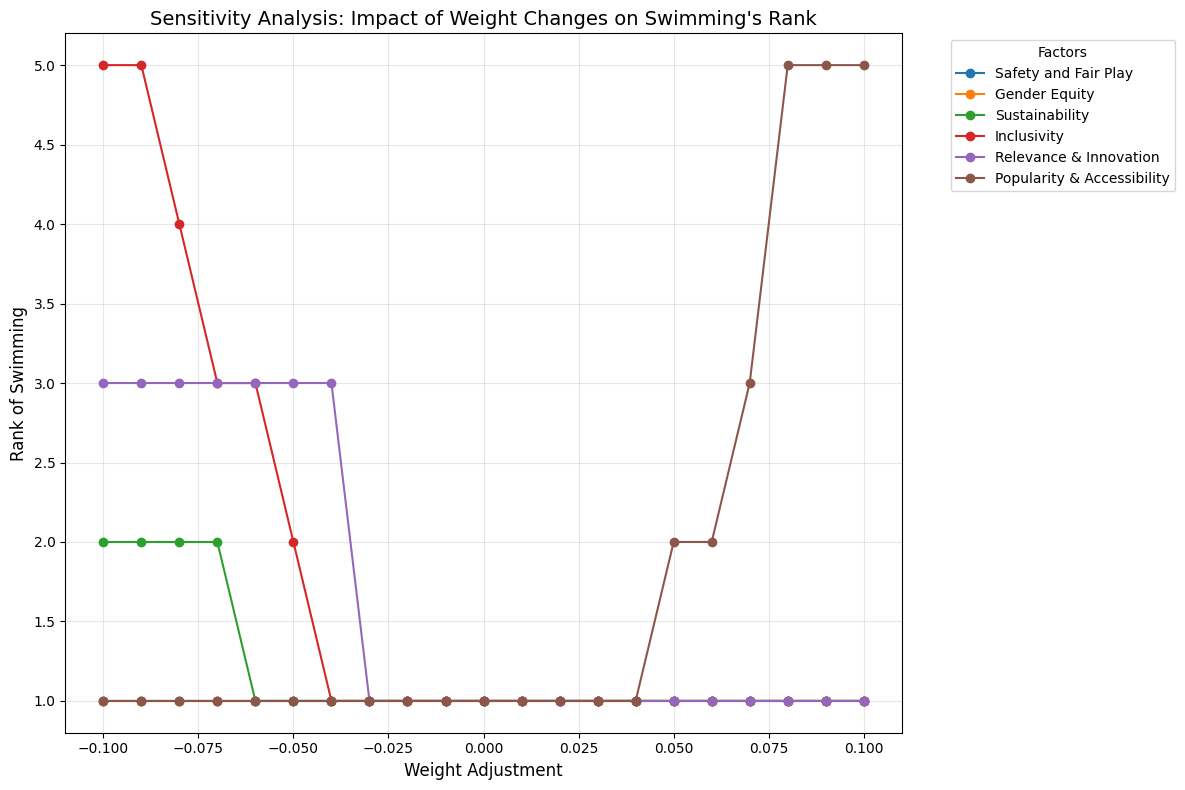
\includegraphics[width=1\textwidth]{Line graph.png}
    \caption{\label{fig:Line graph}}
\end{figure}

\begin{figure}[H]
    \centering
    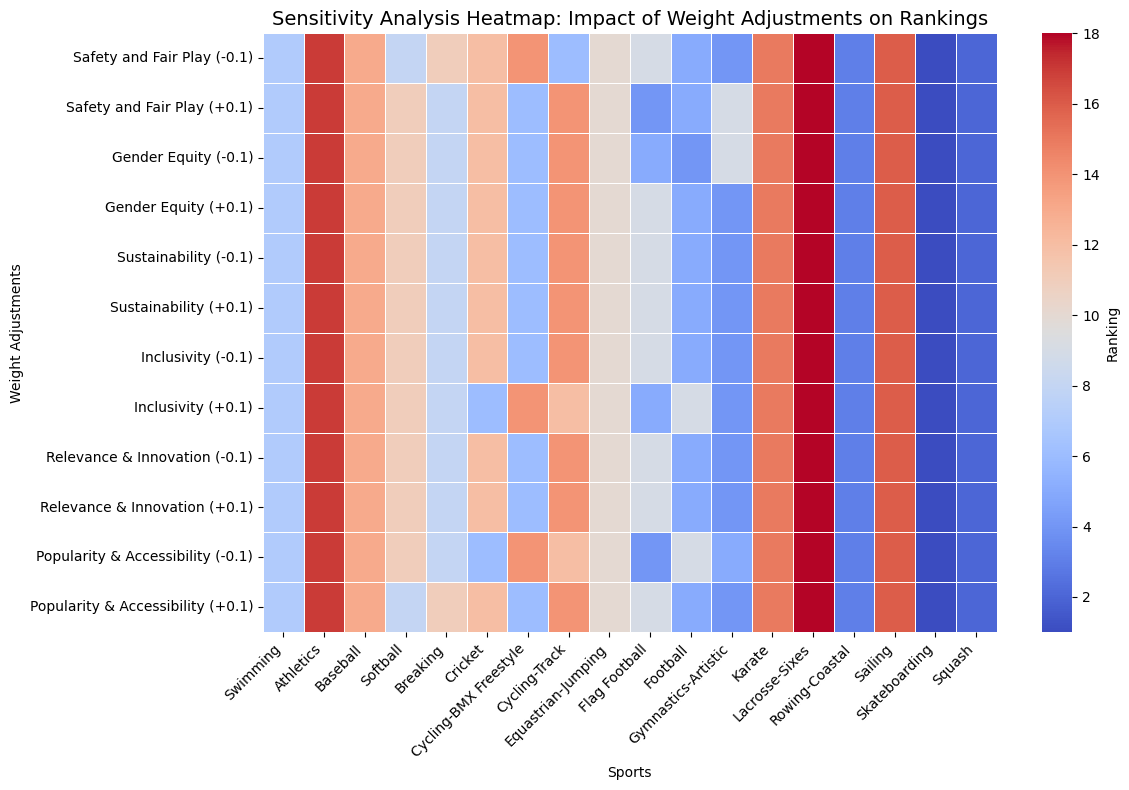
\includegraphics[width=0.7\textwidth]{heatmap.png}
    \caption{\label{fig:Word heatmap}}
\end{figure}

The line chart clearly demonstrates the ranking sensitivity of Swimming to individual weight changes, while the heatmap visualizes ranking fluctuations across all sports disciplines.

\begin{itemize}
    \item An over-reliance on "Popularity and Accessibility," suggesting a need to rebalance weights to achieve more equitable results.

    \item Minimal impact of factors like "Sustainability" and "Gender Equity," indicating a need for higher weights to reflect their importance.

    \item High sensitivity in modern sports like Breaking, which may require additional criteria to stabilize their rankings.
\end{itemize}
\subsection{Robustness Analysis}
\textbf{Introduction}
Robustness analysis tests how stable the model is under real-world uncertainties, such as data inaccuracies or random perturbations. By introducing ±5\% random noise to input data, this analysis simulates potential data inaccuracies to evaluate the stability of rankings and detect sports disciplines that are particularly sensitive to data variability.

\textbf{Methodology}
The analysis involved injecting random noise into the input data and running 100 simulations to compute perturbed rankings. Consistency between baseline rankings and perturbed rankings was measured using Spearman correlation.


The output of the code is as follows:
\begin{itemize}
    \item Average Spearman Correlation: 0.959
    \item Standard Deviation of Spearman Correlation: 0.018
\end{itemize}

\begin{figure}[H]
    \centering
    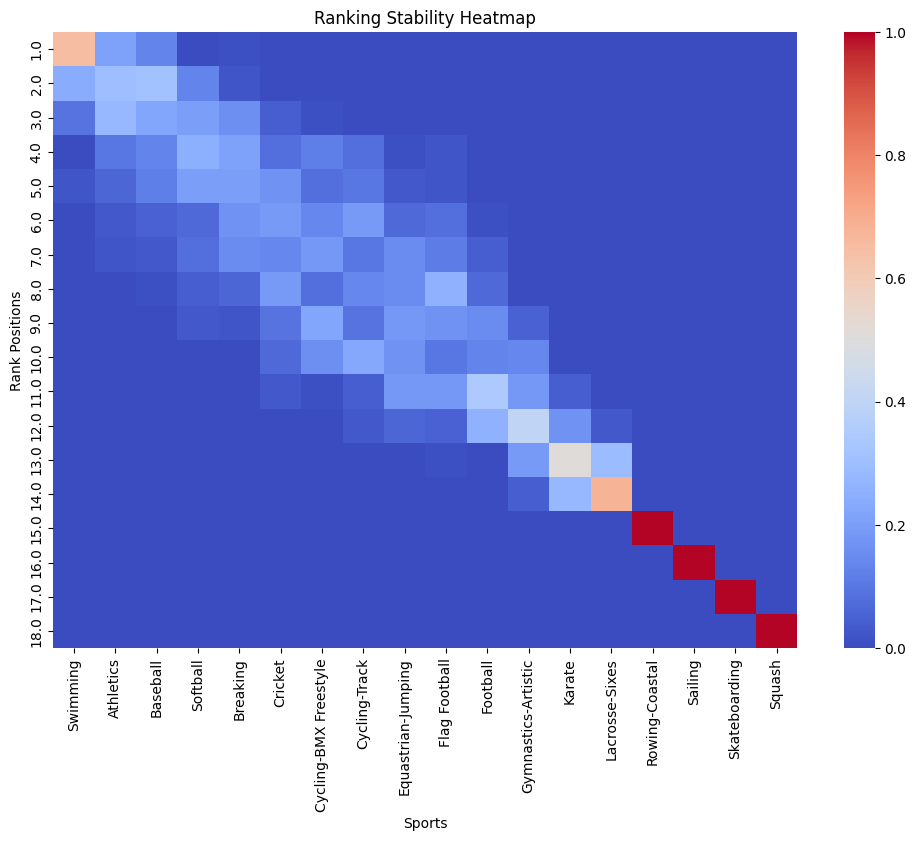
\includegraphics[width=0.6\textwidth]{Rank heatmap.png}
    \caption{\label{fig:Rank heatmap} }
\end{figure}

\textbf{Results}
Robustness analysis confirmed the model’s stability:
\begin{itemize}
    \item The average Spearman correlation between baseline and perturbed rankings was 0.96, with a standard deviation of 0.018, indicating strong consistency.
    \item The average Spearman correlation between baseline and perturbed rankings was 0.96, with a standard deviation of 0.018, indicating strong consistency.
    \item Modern sports, such as Breaking, exhibited greater variability under perturbations, highlighting their sensitivity to input data changes.

\end{itemize}
\begin{comment}\subsubsection{Overall Evaluation}

\begin{enumerate}
    \item \textbf{Sensitivity Analysis:} The factor "Popularity \& Accessibility" dominated ranking adjustments, while "Sustainability" and "Gender Equity" had limited influence. Modern sports were more sensitive to weight changes.
    
    \item \textbf{Robustness Analysis:} The model demonstrated high stability with an average Spearman correlation of 0.96, though modern sports showed greater ranking variability.
\end{enumerate}\end{comment}
\subsection{Strengths} 
\begin{itemize}
    \item Our modal incorporates data in 14 different Olympic sports from recent Olympics
    
    \item We combined AHP, TOPSIS, and the Entropy Method to achieve a balanced evaluation that reduces individual method biases. The Entropy Method specifically counterbalances the subjectivity inherent in AHP, while TOPSIS provides a systematic ranking approach based on ideal solutions.

    \item Our model evaluates SDEs across six factors to ensure all key aspects of Olympic eligibility are considered.

    \item Our app model showcases objectivity, as it is arrived at by gathering the rating of all group members, not an individual.

    \item Our scoring system adapts to existing Olympic sports and potential new additions, accommodating different types of sports and varying data availability.

\end{itemize}
\subsection{Weakness}
\begin{itemize}
    \item \textbf{Absence of authority when evaluating the weights of 6 factors: } 
    Although we obtained the opinion of all four of our group members when applying the AHP analysis, our opinion on the importance of the factors may vary from IOC’s criteria due to our personal values. 

    \item \textbf{Lack of regional considerations: } 
    Certain traits of specific sports may be closely linked to regions and countries. For example, gender equality may have different representations in different countries, and other sports (such as Karate) may have special importance to their country and people. 

    \item \textbf{Limited case and time-sensitivity:}
    Our model heavily relies on historical data of past Olympic events, so we may overlook the possibility of the SDE’s improved performance in the future. Also, with the SDE’s that lack previous data from the Olympics, we looked into other major sports competitions of that sport or the general data sets of athletes engaged in the sports. These circumstances, however, may have variations from that of the Olympics.  

\end{itemize}
\begin{comment}
\section{Conclusion}
In this paper, our team developed a mathematical model to provide a comprehensive evaluation of a Sport, Discipline, or Event (SDE). Because of the importance of the Olympics as a global event and the world’s modernization, many factors must be taken into consideration. Our team used the criteria that IOC has given and converted them into tangible factors that are used to calculate an SDE’s overall alignment to the IOC’s standards. Our factors are: inclusivity, popularity and accessibility, safety and fair play, sustainability, relevance and innovation, and gender equity. Our model is able to provide well-rounded and thoughtful decision-making guidance to the IOC when deciding the inclusion of SDEs in the 2032 Brisbane Games.
\end{comment}

\section{Letter to IOC}
Dear International Olympic Committee (IOC),

        We’re honored to share our recommendations for Sports, Disciplines, and Events (SDEs) for consideration in the 2032 Summer Olympics in Brisbane. We developed a structured approach to assess how well the selected SDEs align with the Olympic criteria: safety, fair play, gender equity, inclusivity, sustainability, popularity, accessibility, relevance, and innovation. Our model is able to provide well-rounded and thoughtful decision-making guidance to the IOC when deciding the inclusion of SDEs in the 2032 Brisbane Games.
        
        First, we assessed the importance of each criterion and calculated their weights using proven methods. This ensured that the factors we prioritized reflected the core values of the Olympics. Then, we scored past and potential SDEs against these criteria, using a consistent scoring system to determine how well each sport matches the Olympic vision. We employed these approaches to make our model reliable and realistic.
        
        Our analysis revealed that while the majority of the SDEs' scores aligned with their current status, karate scored higher than expected. This is because the advantageous data used for the calculation was from the Tokyo 2020 Games, and because karate is culturally Japanese, we believe this led to biased data, causing karate's score to be disproportionately high. When considering the other factors and its actual status, we recommend the removal of karate from the Olympics.
        
        On the other hand, we identified three SDEs that could bring novel experiences to the Brisbane Games, which are pickleball, ultimate frisbee, and bowling (ranked as such). After considerable thought we have established that they adequately fulfill all the criteria, especially prevailing in the realm of popularity. These sports, relatively recent in the world's attention, will constitute an evolutionary step of the Olympics.
        By refining the SDE agenda accordingly, the Brisbane 2032 Games can continue the Olympic legacy while appealing to new generations.
        We are excited to see how our recommendations could shape a more vibrant and inclusive Olympics. Thank you for considering our input, and we are looking forward to seeing the Brisbane Games 2032!
        
Sincerely,

Team 15607

\section{References}
\begin{thebibliography}{99}

\bibitem{euronews} Euronews. Available at: \url{https://www.euronews.com}

\bibitem{bjsm} British Journal of Sports Medicine. Available at: \url{https://bjsm.bmj.com}

\bibitem{healthnews} Health News. Available at: \url{https://healthnews.com}

\bibitem{injuries_pdf} Analysis of Injuries in Competitive Sports. Available at: \url{https://text2fa.ir/wp-content/uploads/Text2fa.ir-Analysis-of-Injuries-in-Competitive.pdf}

\bibitem{injepijournal} Injury Epidemiology Journal. Available at: \url{https://injepijournal.biomedcentral.com}

\bibitem{oup} Oxford Academic. Available at: \url{https://academic.oup.comabstract}

\bibitem{allenpress} Allen Press. Available at: \url{https://meridian.allenpress.com}

\bibitem{mdpi} MDPI Journals. Available at: \url{https://www.mdpi.com}

\bibitem{pickleballunion} Pickleball Union. Available at: \url{https://pickleballunion.com}

\bibitem{dinkpickleball} The Dink Pickleball. Available at: \url{https://www.thedinkpickleball.com}

\bibitem{conwaybulletin} The Conway Bulletin. Available at: \url{https://theconwaybulletin.com}

\bibitem{yorku_library} York University Library. Available at: \url{https://yorkspace.library.yorku.ca}

\bibitem{fide_chennai} FIDE Chennai 2022. Available at: \url{https://chennai2022.fide.com}

\bibitem{sportsfoundation} Sports Foundation. Available at: \url{https://sportsfoundation.org}

\bibitem{sportsdestinations} Sports Destinations. Available at: \url{https://www.sportsdestinations.com}

\bibitem{worldbowls} World Bowls. Available at: \url{https://www.worldbowls.com}

\bibitem{olympics_stillmed} Stillmed Olympics. Available at: \url{https://stillmed.olympics.com}

\bibitem{researchgate} ResearchGate. Available at: \url{https://www.researchgate.net}

\bibitem{wikipedia} Wikipedia. Available at: \url{https://en.wikipedia.org}

\bibitem{olympics} Olympics. Available at: \url{https://olympics.com}

\bibitem{worldaquatics} World Aquatics. Available at: \url{https://www.worldaquatics.com}

\bibitem{worldrowing} World Rowing. Available at: \url{https://worldrowing.com}

\bibitem{theworldgames} The World Games. Available at: \url{https://www.theworldgames.org}

\bibitem{squash_events} Squash Events. Available at: \url{http://sm2022.squash-events.pl}


\bibitem{urbansider} Urban Sider. Available at: \url{https://www.urbansider.com/}

\bibitem{paris2024} Paris 2024 Olympics. Available at: \url{https://olympics.com/en/paris-2024}

\end{thebibliography}

\section{Appendix}

\noindent \textbf{Pseudocode for Google Trends Keyword Web Crawler Results and Analysis}
\begin{Verbatim}[frame=lines, framesep=3mm, framerule=0.5pt]
# Define Sports Keywords and Data Storage Path
Define sports_keywords → Containing keyword list for each sport
Set csv_filename → Path for saving data

# Fetch Google Trends Data
For each sport in sports_keywords:
    → Fetch average interest from Google Trends for associated keywords
    → Append results to data dictionary
    → Save intermediate results to CSV
    → Apply random delay to avoid rate limit

# Load and Preprocess Data
Read collected data from CSV → Fill missing values with median

# Visualization
→ Plot histogram to visualize distribution of average search interest
→ Plot bar chart to rank sports by average interest
\end{Verbatim}



\noindent \textbf{Pseudocode for Data Normalization and Composite Score Calculation}
\begin{Verbatim}[frame=lines, framesep=3mm, framerule=0.5pt]
# Initialize and Merge Data
→ Create DataFrames for Google Trends, attendance, and venue cost
→ Merge DataFrames on "Sport"

# Normalize Data
→ Apply Min-Max normalization to Google Trends, attendance, and cost
→ Calculate accessibility as (1 - normalized cost)

# Set Weights and Calculate Composite Score
→ Set weights for Google Trends, attendance, and accessibility
→ Calculate popularity and accessibility score using weighted sum

# Sort and Visualize Results
→ Sort sports by composite score in descending order
\end{Verbatim}

\noindent \textbf{Pseudocode for Weight Combination Using AHP and Entropy Methods}
\begin{Verbatim}[frame=lines, framesep=3mm, framerule=0.5pt]
# Define Weights
→ Define AHP weights and Entropy weights as pandas Series

# Reorder Weights
→ Reorder AHP weights to match Entropy weights' index

# Calculate Combined Weights
→ Compute geometric mean of AHP and Entropy weights
→ Normalize combined weights to ensure their sum equals 1

# Visualize Combined Weights
→ Plot combined weights as a bar chart
\end{Verbatim}

\noindent \textbf{Pseudocode for Sensitivity Analysis}
\begin{Verbatim}[frame=lines, framesep=3mm, framerule=0.5pt]
# Load Data and Define Weights

# Sensitivity Analysis
→ For each weight:
    → Adjust by +/- 10%
    → Normalize adjusted weights
    → Recalculate and rank scores for each adjustment

\end{Verbatim}

\end{document}




